\documentstyle[11pt,epsfig,fancybox,semcolor,semlayer,doublespace,portrait]
{seminar}
\input clp_utils

\def\ys{$\Upsilon(1S)$}
\def\yss{$\Upsilon(2S)$}
\def\ysss{$\Upsilon(3S)$}
\def\gamee{$\Gamma_{ee}$}
\def\cleo{{\sc Cleo}}
\def\cleoii{{\sc Cleo II}}
\def\cleoiii{{\sc Cleo III}}

% The following strings are needed by the title page and 
% page style definitions in map_utils.tex
\newcommand{\talktitle}[0]{Leptonic Decay Widths \gamee\ of \ys, \yss\ and \ysss}
\newcommand{\fmttitle}[0]{}
\newcommand{\conftitle}[0]{April 2003 Meeting of the American Physical Society}
\newcommand{\myname}[0]{Jim Pivarski}
\newcommand{\affila}[0]{Cornell University}
\newcommand{\talkdate}[0]{April 7, 2003}

\pagestyle{conference}   % From clp_utils.tex

% slide magnification
\slidesmag 1

%%%%%%%%%%%%%%%%%%%%%%%%%%%%%%%%%%%%%%%%%%%%%%%%%%%%%%%%%%%%%%%%%%%%%%%%%%%
% Start document
\begin{document}

% Set page size
\slideheight 7.0in
\slidewidth 8.8in 

% Set array stretch
\renewcommand{\arraystretch}{0.3}
\renewcommand{\slidetopmargin}{0.4in}
\renewcommand{\slidebottommargin}{0.9in}


%%%%%%%%%%%%%%%%%%%%%%%%%%%%%%%%%%%%%%%%%%%%%%%%%%%%%%%%%%%%%%%%%%%%%%%%%%%

\begin{slide*}

\slideframe{}
\slideframe*[\dkblue]{Oval}

\begin{center}
\vspace{4 cm}
{\Huge Leptonic Decay Widths \gamee \\
\vspace{0.25 cm}
of \ys, \yss\  and \ysss}  \\
\vspace{1 cm}
{\LARGE	Jim Pivarski } \\
% \vspace{0.25 cm}
% {\LARGE	Ritchie Patterson } \\
% \vspace{0.25 cm}
% {\LARGE	Karl Berkelman } \\
\vspace{0.25 cm}
{\Large	Cornell University } \\
\vspace{1 cm}
{\LARGE	\cleo\  Collaboration } \\
\vspace{2 cm}
\conftitle \\
{\large \talkdate}

\end{center}

\end{slide*}

% %%%%%%%%%%%%%%%%%%%%%%%%%%%%%%%%%%%%%%%%%%%%%%%%%%%%%%%%%%%%%%%%%%%%%%%%%%%

% \begin{slide*}

% \slideframe{}
% \slideframe*[\dkblue]{Oval}
% \huge
% \heading{Outline}
% \vspace{1 cm}

% \begin{center}
% \begin{minipage}[t]{12 cm}
% \begin{itemize}
% \LARGE \item {\huge Motivation: verify lattice QCD!}
% \LARGE \item {\huge 2 out of 3 Resonances Scanned}
% \LARGE \item {\huge Energy Calibration Systematics}
% \LARGE \item {\huge Other Systematics / Work to be Done}
% \end{itemize}
% \end{minipage}
% \end{center}

% \end{slide*}
 
%%%%%%%%%%%%%%%%%%%%%%%%%%%%%%%%%%%%%%%%%%%%%%%%%%%%%%%%%%%%%%%%%%%%%%%%%%%

\begin{slide*}

\slideframe{}
\slideframe*[\dkblue]{Oval}
\heading{\huge Motivation}

\begin{minipage}[t]{\linewidth}
\Large

\vspace{0.25cm}

$\Gamma(\Upsilon(1S) \to e^+ e^-)$, $\Gamma(\Upsilon(2S) \to e^+ e^-)$,
and $\Gamma(\Upsilon(3S) \to e^+ e^-)$
\mbox{are three} experimental checks on Precision Lattice QCD.

\vspace{0.25cm}

Current precisions are 2\%, 4\% and 9\%, respectively.  This
measurement can reduce them to 2\% each, or better.

\vspace{1cm}

\heading{\huge Measurement Strategy}

\vspace{0.25cm}

\begin{minipage}{1.2\linewidth}
  {\red \gamee} is proportional to {\blue the area
    of the hadronic cross-section peak:}
\end{minipage}

\[ \begin{array}{r c l}
\displaystyle {\red \Gamma(\Upsilon \to e^+ e^-)} &=&
\displaystyle\frac{\mbox{$M_\Upsilon$}^2}{6 \pi^2} \int d\mbox{\sc \small Energy} \, \sigma(e^+ e^- \to \Upsilon) 
\vspace{0.3cm} \\
&=& \displaystyle \frac{\mbox{$M_\Upsilon$}^2}{6 \pi^2}
    \frac{\Gamma_{\mbox{\small total}}}{\Gamma_{\mbox{\small hadrons}}} {\blue \int d\mbox{\sc \small Energy} \,
    \sigma(e^+ e^- \to \Upsilon \to \mbox{\small hadrons})}
\end{array} \]

\vspace{0.25cm}

\begin{center}
  \epsfig{file=cartoon.eps, width=0.85\linewidth}
\end{center}

\end{minipage}

\end{slide*}

% %%%%%%%%%%%%%%%%%%%%%%%%%%%%%%%%%%%%%%%%%%%%%%%%%%%%%%%%%%%%%%%%%%%%%%%%%%%

\begin{slide*}
\slideframe{}
\slideframe*[\dkblue]{Oval}
% \heading{\huge Data}
\begin{minipage}[t]{\linewidth}

%% \begin{picture}\begin{tabular}{p{2.39cm} c c c}
%% %%   &
%% %%   $\frac{\mbox{0.5 fb$^{-1}$}}{\mbox{2/3}}$ = 0.75 fb$^{-1}$ &
%% %%   $\frac{\mbox{0.2 fb$^{-1}$}}{\mbox{1/2}}$ = 0.4 fb$^{-1}$ &
%% %%   0.6 fb$^{-1}$ \\
%%   & 0.75 fb$^{-1}$ \ys & 0.4 fb$^{-1}$ \yss & 0.6 fb$^{-1}$ \ysss \\
%%   & 
%%   \epsfig{file=y1s.eps, width=3.8cm} &
%%   \epsfig{file=y2s.eps, width=3.8cm} &
%%   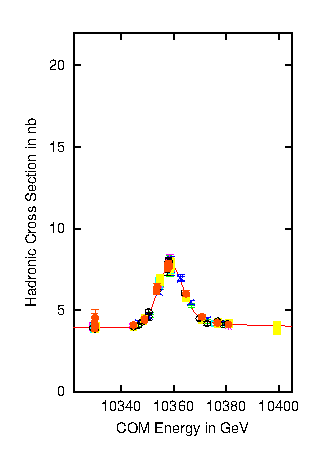
\epsfig{file=y3s.eps, width=3.8cm} \\


%% \end{tabular}\end{picture}

\begin{center}
  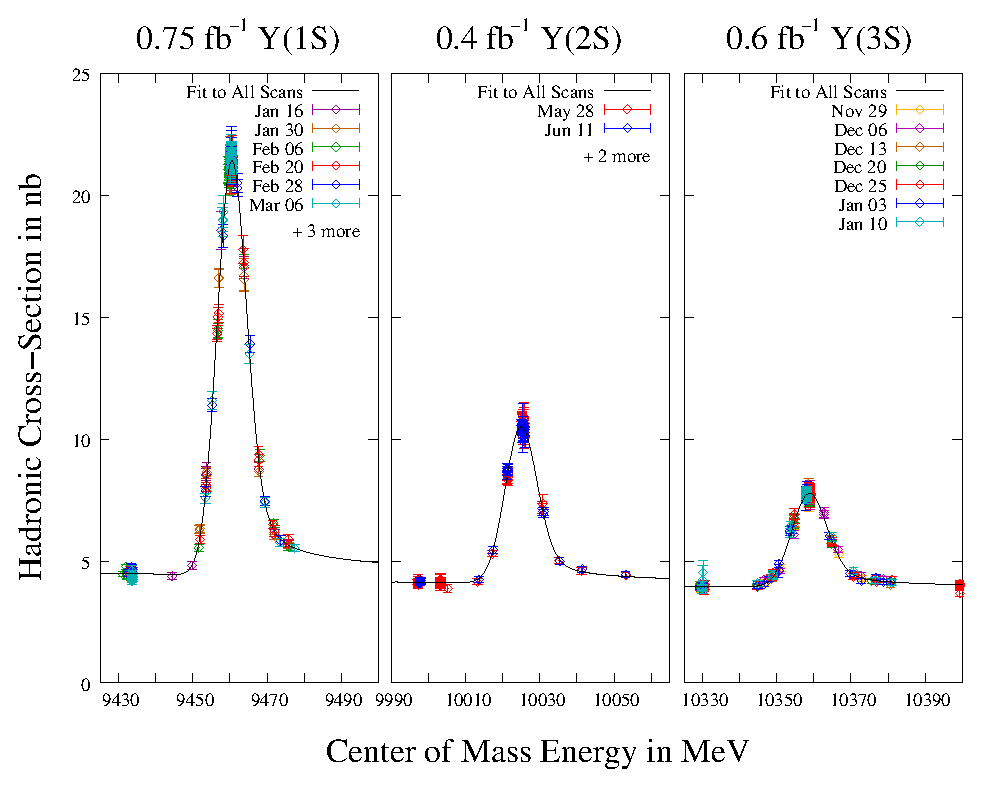
\epsfig{file=allfits2.eps, height=0.95\linewidth, angle=-90}
\end{center}

\end{minipage}
\end{slide*}

% %%%%%%%%%%%%%%%%%%%%%%%%%%%%%%%%%%%%%%%%%%%%%%%%%%%%%%%%%%%%%%%%%%%%%%%%%%%

\begin{slide*}
\slideframe{}
\slideframe*[\dkblue]{Oval}
\heading{\huge Sources of Uncertainty}
\begin{minipage}[t]{\linewidth}
\Large

\vspace{0.25cm}

{\LARGE Statistical uncertainties are 0.1\% to 0.5\%.}

\vspace{0.75cm}

{\LARGE There are four sources of systematic error on \gamee:}

\begin{itemize}

  \item {\LARGE {\bf Energy Calibration} {\it (in progress)}}
    \begin{itemize}

      \item Only beam-energy calibration {\it changes} within
	a 10-hour scan affect \gamee.

      \item None have been seen.

      \item Worst-case effect is $\pm$1.0\%.

    \end{itemize}

  \vspace{0.2cm}

  \item {\LARGE {\bf Acceptance} {\it (planned)}}
    \begin{itemize}
      
      \item Can be measured with $\Upsilon(3S) \to \Upsilon(1S)\, \pi^+ \pi^-$
	(independently of Monte Carlo) to $\pm$0.6\%.

    \end{itemize}

  \vspace{0.2cm}

  \item {\LARGE {\bf Luminosity} {\it (speculated)}}
    \begin{itemize}

      \item Current \cleoiii\ systematic of $\pm$2\% can be improved.

      \item \cleoii\ luminosity systematic was $\pm$1.0\%!

    \end{itemize}

  \vspace{0.2cm}

  \item {\LARGE {\bf Backgrounds} {\it (nearly finished!)}}
    \begin{itemize}

      \item Measured to be $\pm$0.3\%.

    \end{itemize}

\end{itemize}

\end{minipage}
\end{slide*}

% %%%%%%%%%%%%%%%%%%%%%%%%%%%%%%%%%%%%%%%%%%%%%%%%%%%%%%%%%%%%%%%%%%%%%%%%%%%

\begin{slide*}
\slideframe{}
\slideframe*[\dkblue]{Oval}
\heading{\huge Sources of Background}
\begin{minipage}[t]{\linewidth}

\vspace{0.25cm}
\hspace{-0.25cm}
\begin{center}
  \epsfig{file=plot_em_all3.eps, width=\linewidth}
\end{center}

\end{minipage}
\end{slide*}

% %%%%%%%%%%%%%%%%%%%%%%%%%%%%%%%%%%%%%%%%%%%%%%%%%%%%%%%%%%%%%%%%%%%%%%%%%%%

\begin{slide*}
\slideframe{}
\slideframe*[\dkblue]{Oval}
\heading{\huge Cutting/Counting Beam-Gas Contamination}
\begin{minipage}[t]{\linewidth}
\Large

\vspace{0.01cm}

1.\ Require that the primary vertex be near the beam spot.
\begin{center}
  \vspace{-0.25cm} 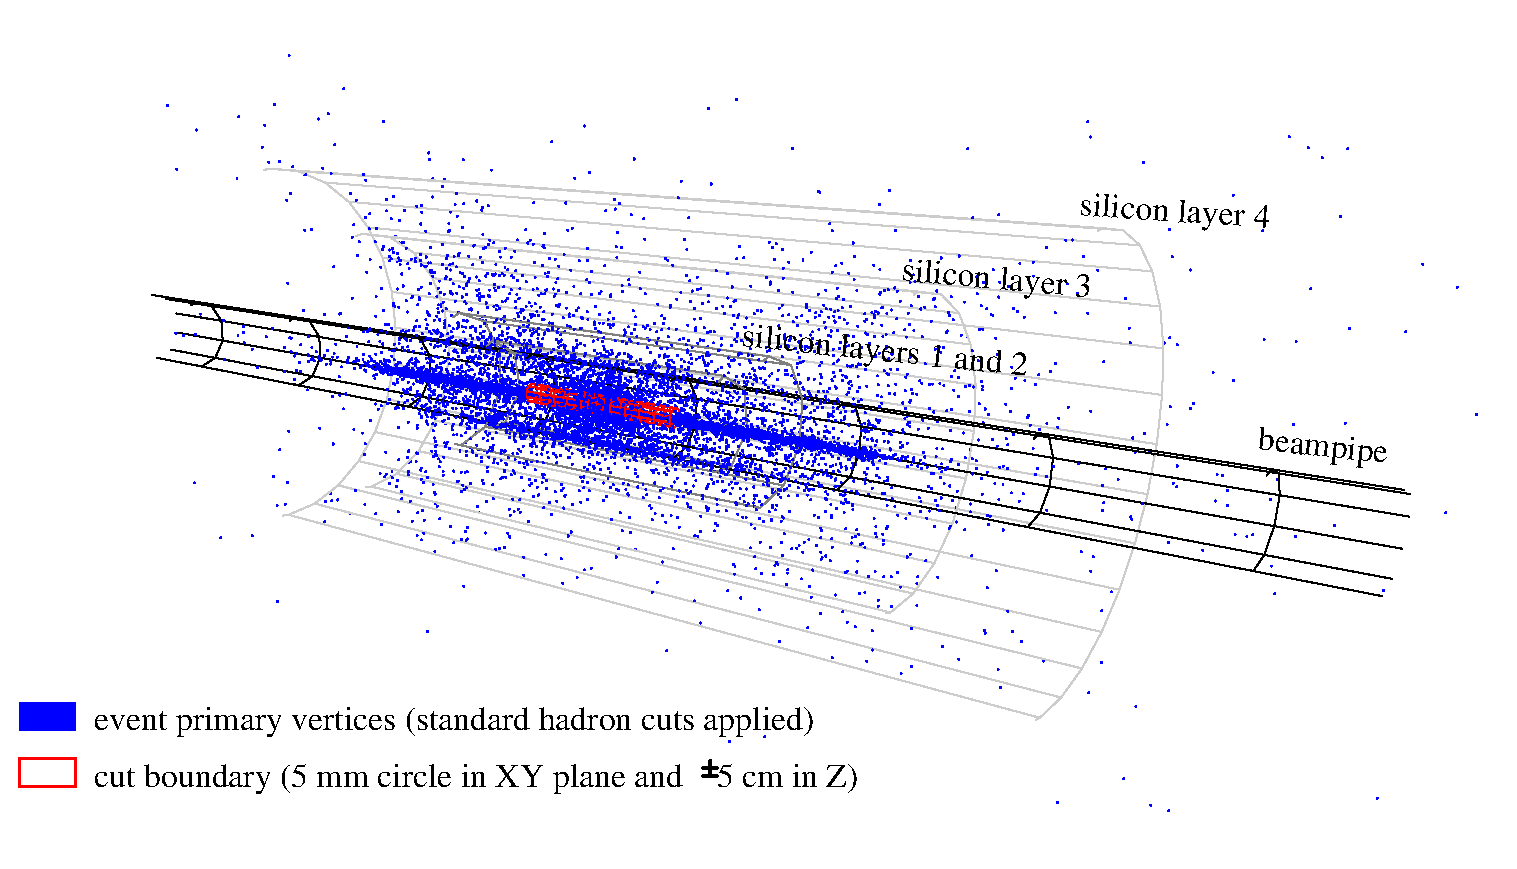
\epsfig{file=cuts_illustration4.eps, width=0.9\linewidth} \vspace{-1.1cm}\\
  \hspace{-1cm} \begin{tabular}{l r}
    \begin{minipage}{0.7\linewidth}
      \epsfig{file=determine_factor2.eps, width=\linewidth}
    \end{minipage}
    \begin{minipage}{0.2\linewidth}
      \setlength{\baselineskip}{1.5\baselineskip}
      \raggedright
      \mbox{2.\ Extrapolate} beam-gas events (which extend to $\pm$20 cm in Z)
      into the cut region.
    \end{minipage}
  \end{tabular}
\end{center}

\end{minipage}
\end{slide*}

% %%%%%%%%%%%%%%%%%%%%%%%%%%%%%%%%%%%%%%%%%%%%%%%%%%%%%%%%%%%%%%%%%%%%%%%%%%%

%% \begin{slide*}
%% \slideframe{}
%% \slideframe*[\dkblue]{Oval}
%% \heading{\huge Measuring the Remaining Beamgas Contamination}
%% \begin{minipage}[t]{\linewidth}
%% \Large

%% \vspace{0.25cm}

%% Collision events are confined to a Z primary vertex of $\pm$ 5 cm, while
%% beamgas reaches $\pm$ 20 cm.

%% \vspace{0.25cm}

%% A special ``single-beam'' data sample was taken in which only one beam
%% was present in the machine ($e^+$ only or $e^-$ only).  All event
%% selection was the same.

%% \vspace{-1cm}

%%     \hspace{-1cm}
%%     \begin{minipage}{0.25\linewidth}
%%       \raggedright
%%       From the \\
%%       \vspace{0.2cm}
%%       \vspace{0.4cm}
%%       $\displaystyle \frac{\mbox{center beamgas}}{\mbox{shoulder beamgas}}$ \\
%%       \vspace{0.2cm}
%%       \vspace{0.4cm}
%%       ratio, we can \\
%%       \vspace{0.4cm}
%%       project the \\
%%       \vspace{0.4cm}
%%       data beamgas \\
%%       \vspace{0.4cm}
%%       distribution into \\
%%       \vspace{0.4cm}
%%       the cut region \\
%%       \vspace{0.4cm}
%%       for subtraction.
%%     \end{minipage}
%%     \\


%% \end{minipage}
%% \end{slide*}

% %%%%%%%%%%%%%%%%%%%%%%%%%%%%%%%%%%%%%%%%%%%%%%%%%%%%%%%%%%%%%%%%%%%%%%%%%%%

\begin{slide*}
\slideframe{}
\slideframe*[\dkblue]{Oval}
\heading{\huge Simulating Continuum $q\bar{q}$ Interference}
\begin{minipage}[t]{\linewidth}
\Large

\vspace{0.5cm}

A fraction of the $\Upsilon \to$ hadrons events can interfere with the
\mbox{continuum} background:

\vspace{0.25cm}
\begin{center}
  \epsfig{file=qqbar_interference.eps, height=2.5cm}
\end{center}

\vspace{0.5cm}

%% The phase of the non-resonant part is nearly constant with respect to
%% energy, but the phase of the resonance cycles 180$^\circ$ through the
%% resonance peak.

%% \[
%%   \arg\left\{\frac{\Gamma}{\mbox{\sc Energy} - M_\Upsilon + i\Gamma/2}\right\} =
%%   \tan^{-1}\left(\frac{\Gamma/2}{\mbox{\sc Energy} - M_\Upsilon}\right)
%% \]

Cross-term is:
\[
  2 \Gamma M_\Upsilon \sqrt{\frac{{\mathcal B}_{\Upsilon \to q\bar{q}} \,
  \sigma_{\mbox{\small continuum}}}{6 \pi^2 \Gamma_{ee} \Gamma_{\mbox{\small hadrons}}}} \,
  \left(\frac{\mbox{\sc Energy} - M_\Upsilon}{\Gamma}\right)
  \times \sigma_{\mbox{\small Breit-Wigner}}(\mbox{\sc Energy})
\]
or about 5\% of the Breit-Wigner cross-section.

\vspace{0.5cm}

\begin{center}
  {\bf \normalsize Fit Function with Greatly Exaggerated Cross-Term}
  \epsfig{file=bigyint_lineshape.eps, width=0.7\linewidth}
\end{center}

\end{minipage}
\end{slide*}

% %%%%%%%%%%%%%%%%%%%%%%%%%%%%%%%%%%%%%%%%%%%%%%%%%%%%%%%%%%%%%%%%%%%%%%%%%%%

\begin{slide*}
\slideframe{}
\slideframe*[\dkblue]{Oval}
\heading{\huge Table of All Uncertainties}
\begin{minipage}[t]{\linewidth}
\large

\vspace{0.25cm}

\hspace{-0.2cm} \begin{minipage}{\linewidth}
  \begin{tabular}{p{4.0cm} c c c}
    & {\LARGE \ys} & {\LARGE \yss} & {\LARGE \ysss} \vspace{0.25cm} \\

    \mbox{\LARGE Contribution to Uncertainty in yield (and \gamee):} & & & \\
    Beam-gas & 0.04\% & 0.02\% & 0.05\% \\
    Beam-wall & zero & zero & zero \\
    Cosmic Rays & 0.003\% & 0.001\% & 0.003\% \\
    Two-Photon Process & 0.02\% & 0.04\% & 0.03\% \\
    $J/\psi$ and $\Upsilon$ ISR tails & 0.0006\% & 0.05\% & 0.03\% \\
    $\Upsilon \to \tau^+ \tau^-$ & 0.02\% & 0.07\% & 0.04\% \\
    \raggedright $e^+ e^- \to \tau^+ \tau^-$ \mbox{\hspace{0.65cm} interference} & 0.09\% & 0.08\% & 0.04\% \\
    \raggedright $e^+ e^- \to q\bar{q}$ \mbox{\hspace{0.65cm} interference} & $\sim$0.3\% & $\sim$0.3\% & $\sim$0.3\% \\\hline
    \mbox{\hspace{-0.1cm}\epsfig{file=hilight, width=14.5cm}} & & & \vspace{-0.85cm}\\
    Sum of Backgrounds: & 0.32\% & 0.33\% & 0.31\% \vspace{0.5cm} \\

    Statistics & 0.13\% & 0.30\% & 0.48\% \vspace{0.5cm} \\

    \mbox{\LARGE {\it Predicted} Contributions:} & & & \\
    Energy Stability & $<$ 0.6\% & $<$ 1.0\% & $<$ 0.9\% \\
    Acceptance & $\sim$ 0.6\% & $\sim$ 0.6\% & $\sim$ 0.6\% \\
    Luminosity & $\sim$ 2\% & $\sim$ 2\% & $\sim$ 2\% \vspace{0.25cm}\\\hline
    & & & \vspace{-0.35cm}\\

    \mbox{\hspace{-0.1cm}\epsfig{file=hilight2, width=14.5cm}} & & & \vspace{-0.9cm}\\
    \mbox{\LARGE Predicted Totals:} & \mbox{2.2\%} & \mbox{2.4\%} & \mbox{2.3\%} \vspace{0.5cm} \\

    PDG Best Value
    & \hspace{0.95cm} 3.3\% {\small ({\sc Novo} '96)} \hspace{-0.95cm} 
    & \hspace{0.95cm} 6.4\% {\small ({\sc Novo} '96)} \hspace{-0.95cm} 
    & \hspace{0.9cm} 9.4\% {\small ({\sc Cleo} '84)} \hspace{-0.9cm} \\
    PDG Average & 2.2\% & 4.1\% & 9.4\% \\

  \end{tabular}
\end{minipage}

\end{minipage}
\end{slide*}

% %%%%%%%%%%%%%%%%%%%%%%%%%%%%%%%%%%%%%%%%%%%%%%%%%%%%%%%%%%%%%%%%%%%%%%%%%%%

\begin{slide*}
\slideframe{}
\slideframe*[\dkblue]{Oval}
\heading{\huge Conclusion: What This Means for Lattice QCD}
\begin{minipage}[t]{\linewidth}
\Large

\vspace{0.5cm}

First data/theory comparison: in the $\displaystyle
  \frac{\Gamma_{ee}(2S)}{\Gamma_{ee}(1S)}$ ratios, acceptance and
  luminosity \mbox{corrections} cancel, yielding smaller
  uncertainties.

\vspace{0.5cm}

Some theory errors cancel as well.

\vspace{0.5cm}

\begin{center}
  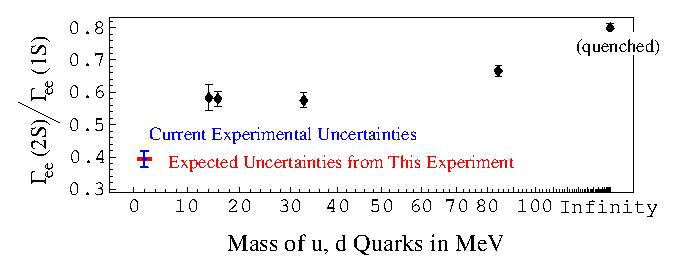
\epsfig{file=conclusion.eps, width=\linewidth}
\end{center}

\vspace{0.5cm}

Theory points by Christine Davies and Alan Gray of the University of
Glasgow, and used with their permission.  (Thank you!)

\end{minipage}
\end{slide*}

% %%%%%%%%%%%%%%%%%%%%%%%%%%%%%%%%%%%%%%%%%%%%%%%%%%%%%%%%%%%%%%%%%%%%%%%%%%%

\begin{slide*}
\slideframe{}
\slideframe*[\dkblue]{Oval}
\heading{\huge Energy Stability}
\begin{minipage}[t]{\linewidth}
\Large

\vspace{0.25cm}

CESR beam energy measured by two NMR magnetic field probes in test
magnets in series with the beam magnets.
\vspace{0.4cm}

%% Scans are protected against long-term drifts in beam energy
%% calibration because they were short (10 hours each).
%% \vspace{0.4cm}

\begin{tabular}{l c r}
  \begin{minipage}{0.5\linewidth}

  \begin{center}
    \epsfig{file=energy_order.eps, width=\linewidth}
  \end{center}

  \setlength{\baselineskip}{1.2\baselineskip}

  \vspace{0.5cm}

  To measure {\it any possible} jitter in calibration during a scan,
  some scans repeated a point of high slope.  Early/late agreement can
  be translated into beam energy measurement errors.

  \vspace{0.5cm}

  \end{minipage}
  & \hspace{0.2cm} &
  \begin{minipage}{0.38\linewidth}
    \begin{center}
      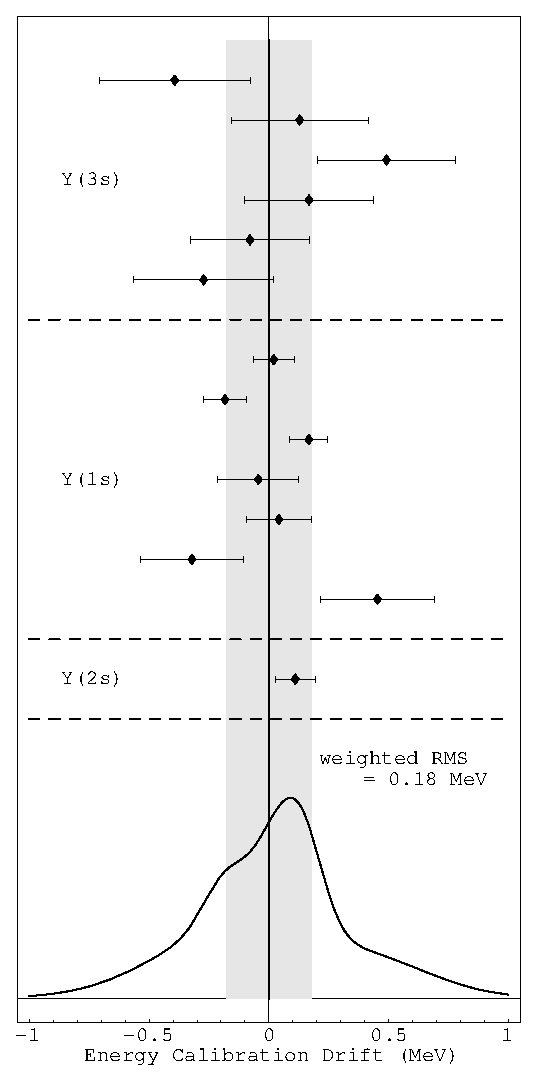
\epsfig{file=all_consistency.eps, width=\linewidth}
    \end{center}
  \end{minipage}
\end{tabular}
\vspace{0.25cm} \\

Deviations are dominated by statistical fluctuations, which place an
upper limit of $\Delta E_{\mbox{\normalsize Calibration}} <$ 0.2 MeV.

\end{minipage}
\end{slide*}

% %%%%%%%%%%%%%%%%%%%%%%%%%%%%%%%%%%%%%%%%%%%%%%%%%%%%%%%%%%%%%%%%%%%%%%%%%%%

\begin{slide*}
\slideframe{}
\slideframe*[\dkblue]{Oval}
\heading{\huge Hadron Selection Criteria}
\begin{minipage}[t]{\linewidth}
\Large

\vspace{0.2cm}

\begin{itemize}

  \item Keep 95\% of hadrons

  \item Keep 0.2\% of beamgas/beamwall/cosmics

  \item Keep 0.09\% of bhabhas

\end{itemize}

\begin{center}
  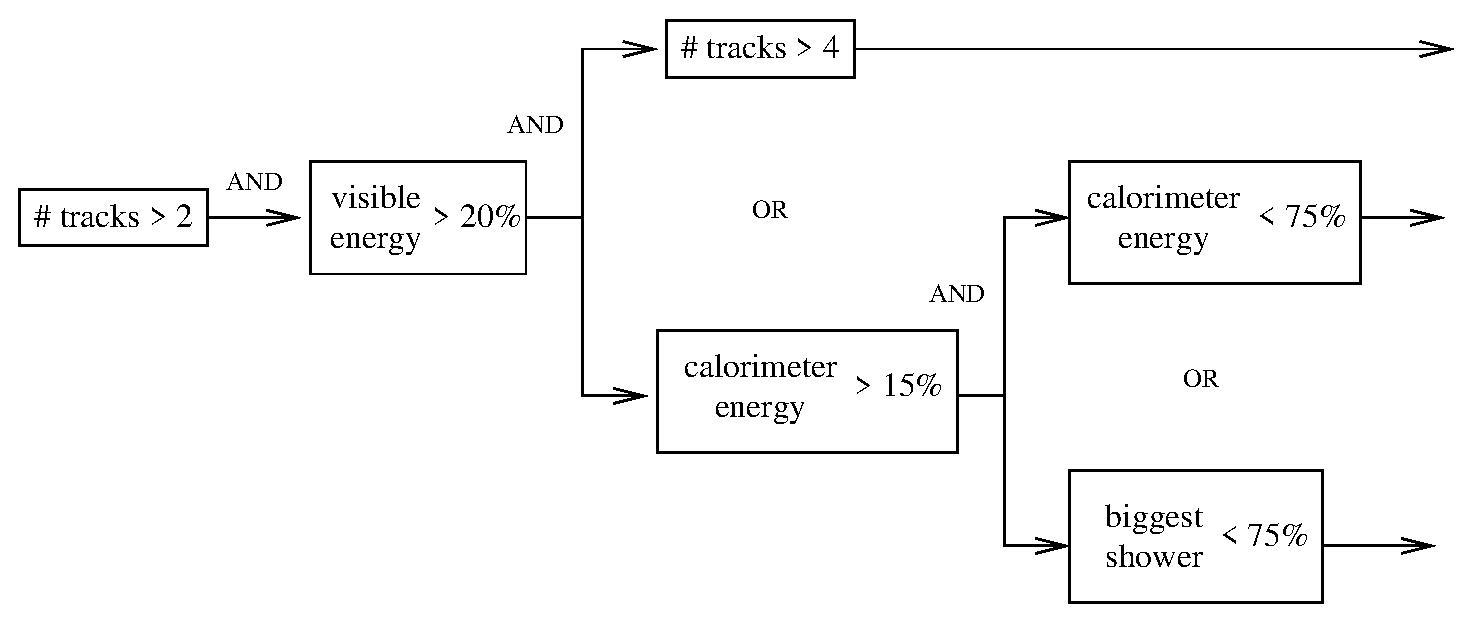
\epsfig{file=hadron.eps, width=\linewidth} \\
  \vspace{0.5cm}
  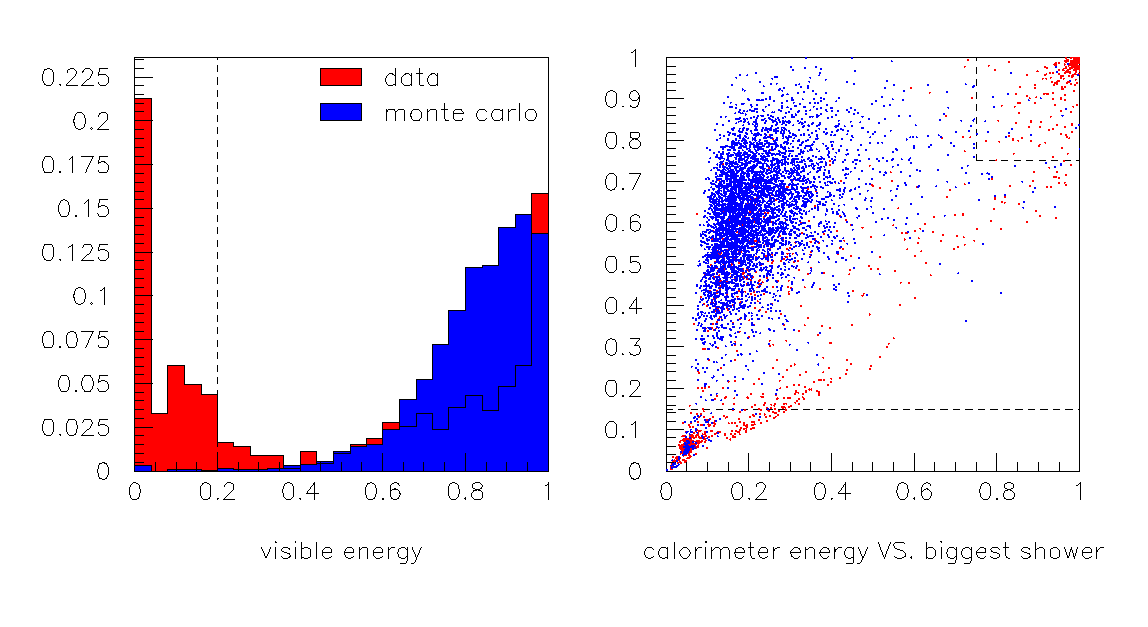
\epsfig{file=subcollectioncuts.eps, width=\linewidth} \\
\end{center}

\end{minipage}
\end{slide*}

% %%%%%%%%%%%%%%%%%%%%%%%%%%%%%%%%%%%%%%%%%%%%%%%%%%%%%%%%%%%%%%%%%%%%%%%%%%%

\begin{slide*}
\slideframe{}
\slideframe*[\dkblue]{Oval}
\heading{\huge Plan for Measuring Acceptance}
\begin{minipage}[t]{\linewidth}
\Large

\vspace{0.25cm}

Procedure:
\begin{enumerate}

  \item Identify $\Upsilon(3S) \to \Upsilon(1S)\  \pi^+ \pi^-$ events by the two pions.

  \item Remove the pions from the event.

  \item Apply all cut criteria on the rest of the event.

\end{enumerate}

\vspace{0.5cm}

\begin{center}
  \epsfig{file=dipion2.eps, width=\linewidth}
\end{center}

\vspace{0.5cm}

Efficiency can be calculated as
\[ \epsilon = 1 - \frac{\mbox{events that fail cut: }
(\mbox{in peak} - \mbox{in side-band})}{\mbox{events: }
(\mbox{in peak} - \mbox{in side-band})} \]

\vspace{0.5cm}

For 95\%--efficient cuts, statistical uncertainty is 0.6\%.

\end{minipage}
\end{slide*}

% %%%%%%%%%%%%%%%%%%%%%%%%%%%%%%%%%%%%%%%%%%%%%%%%%%%%%%%%%%%%%%%%%%%%%%%%%%%

% \begin{slide*}
% \slideframe{}
% \slideframe*[\dkblue]{Oval}
% \heading{\huge REPLACEME}
% \begin{minipage}[t]{\linewidth}

% \end{minipage}
% \end{slide*}

% %%%%%%%%%%%%%%%%%%%%%%%%%%%%%%%%%%%%%%%%%%%%%%%%%%%%%%%%%%%%%%%%%%%%%%%%%%%

% \begin{slide*}
% \slideframe{}
% \slideframe*[\dkblue]{Oval}
% \heading{\huge REPLACEME}
% \begin{minipage}[t]{\linewidth}

% \end{minipage}
% \end{slide*}

% %%%%%%%%%%%%%%%%%%%%%%%%%%%%%%%%%%%%%%%%%%%%%%%%%%%%%%%%%%%%%%%%%%%%%%%%%%%

% \begin{slide*}
% \slideframe{}
% \slideframe*[\dkblue]{Oval}
% \heading{\huge REPLACEME}
% \begin{minipage}[t]{\linewidth}

% \end{minipage}
% \end{slide*}

% %%%%%%%%%%%%%%%%%%%%%%%%%%%%%%%%%%%%%%%%%%%%%%%%%%%%%%%%%%%%%%%%%%%%%%%%%%%

% \begin{slide*}
% \slideframe{}
% \slideframe*[\dkblue]{Oval}
% \heading{\huge REPLACEME}
% \begin{minipage}[t]{\linewidth}

% \end{minipage}
% \end{slide*}

% %%%%%%%%%%%%%%%%%%%%%%%%%%%%%%%%%%%%%%%%%%%%%%%%%%%%%%%%%%%%%%%%%%%%%%%%%%%

% \begin{slide*}
% \slideframe{}
% \slideframe*[\dkblue]{Oval}
% \heading{\huge REPLACEME}
% \begin{minipage}[t]{\linewidth}

% \end{minipage}
% \end{slide*}

% %%%%%%%%%%%%%%%%%%%%%%%%%%%%%%%%%%%%%%%%%%%%%%%%%%%%%%%%%%%%%%%%%%%%%%%%%%%

% \begin{slide*}
% \slideframe{}
% \slideframe*[\dkblue]{Oval}
% \heading{\huge REPLACEME}
% \begin{minipage}[t]{\linewidth}

% \end{minipage}
% \end{slide*}

% %%%%%%%%%%%%%%%%%%%%%%%%%%%%%%%%%%%%%%%%%%%%%%%%%%%%%%%%%%%%%%%%%%%%%%%%%%%

% \begin{slide*}
% \slideframe{}
% \slideframe*[\dkblue]{Oval}
% \heading{\huge REPLACEME}
% \begin{minipage}[t]{\linewidth}

% \end{minipage}
% \end{slide*}

% %%%%%%%%%%%%%%%%%%%%%%%%%%%%%%%%%%%%%%%%%%%%%%%%%%%%%%%%%%%%%%%%%%%%%%%%%%%

% \begin{slide*}
% \slideframe{}
% \slideframe*[\dkblue]{Oval}
% \heading{\huge REPLACEME}
% \begin{minipage}[t]{\linewidth}

% \end{minipage}
% \end{slide*}

% %%%%%%%%%%%%%%%%%%%%%%%%%%%%%%%%%%%%%%%%%%%%%%%%%%%%%%%%%%%%%%%%%%%%%%%%%%%

% \begin{slide*}
% \slideframe{}
% \slideframe*[\dkblue]{Oval}
% \heading{\huge REPLACEME}
% \begin{minipage}[t]{\linewidth}

% \end{minipage}
% \end{slide*}

% %%%%%%%%%%%%%%%%%%%%%%%%%%%%%%%%%%%%%%%%%%%%%%%%%%%%%%%%%%%%%%%%%%%%%%%%%%%

% \begin{slide*}
% \slideframe{}
% \slideframe*[\dkblue]{Oval}
% \heading{\huge REPLACEME}
% \begin{minipage}[t]{\linewidth}

% \end{minipage}
% \end{slide*}

% %%%%%%%%%%%%%%%%%%%%%%%%%%%%%%%%%%%%%%%%%%%%%%%%%%%%%%%%%%%%%%%%%%%%%%%%%%%

% \begin{slide*}
% \slideframe{}
% \slideframe*[\dkblue]{Oval}
% \heading{\huge REPLACEME}
% \begin{minipage}[t]{\linewidth}

% \end{minipage}
% \end{slide*}

% %%%%%%%%%%%%%%%%%%%%%%%%%%%%%%%%%%%%%%%%%%%%%%%%%%%%%%%%%%%%%%%%%%%%%%%%%%%

% \begin{slide*}
% \slideframe{}
% \slideframe*[\dkblue]{Oval}
% \heading{\huge REPLACEME}
% \begin{minipage}[t]{\linewidth}

% \end{minipage}
% \end{slide*}

% %%%%%%%%%%%%%%%%%%%%%%%%%%%%%%%%%%%%%%%%%%%%%%%%%%%%%%%%%%%%%%%%%%%%%%%%%%%

% \begin{slide*}
% \slideframe{}
% \slideframe*[\dkblue]{Oval}
% \heading{\huge REPLACEME}
% \begin{minipage}[t]{\linewidth}

% \end{minipage}
% \end{slide*}

% %%%%%%%%%%%%%%%%%%%%%%%%%%%%%%%%%%%%%%%%%%%%%%%%%%%%%%%%%%%%%%%%%%%%%%%%%%%

% \begin{slide*}
% \slideframe{}
% \slideframe*[\dkblue]{Oval}
% \heading{\huge REPLACEME}
% \begin{minipage}[t]{\linewidth}

% \end{minipage}
% \end{slide*}

\end{document}

